\documentclass[14pt,fleqn]{extarticle}
\RequirePackage{prepwell}
\previewoff
\begin{document}

\newcommand\intg{\int_{-1}^2}

%text
Using integration, find the area bounded by
the curves $x^2 = 4y$ and the line $x = 4y-2$
%

\newcard

From just the equations of the curves, we can infer the following 
\begin{center}
  \begin{tabular}{NlN}
   \toprule
        \text{Curve} & Shape & \text{Why?} \\
   \midrule 
   x^2 = 4y & Parabola facing up & y \geq 0\,\forall x\\
    \midrule 
    x = 4y-2 & Positive sloping line & y = \frac{x}{4} + \frac{1}{2}  \\
    & & \implies m = \frac{1}{4} \\
    \bottomrule
  \end{tabular}
\end{center}

Moreover, the parabola goes through $(0,0)$ and the line cuts the $y-$axis at $\left(0, \frac{1}{2} \right)$\newline 

Hence, the two curves and the required area $A$ are as shown below 

\begin{center}
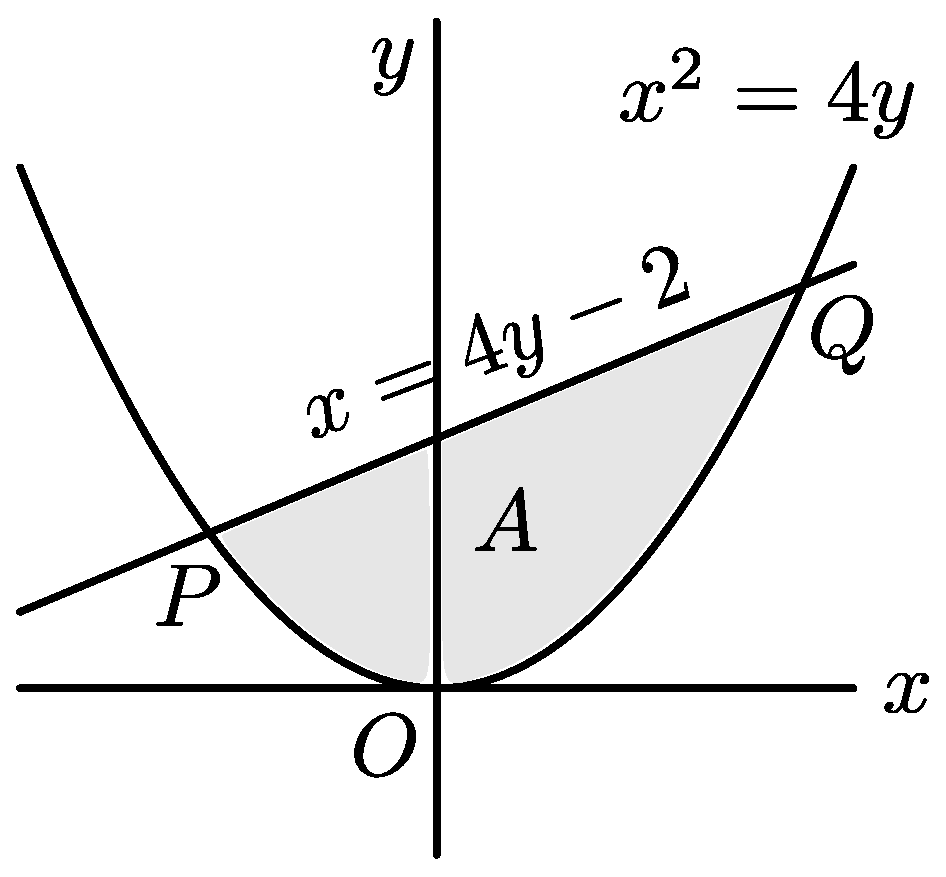
\includegraphics[scale=0.3]{figure.eps} 
\end{center} 


\newcard

The two curves intersect at 
\begin{align}
P &= \left( -1, \dfrac{1}{4}\right)  \text{ and } Q = \left( 2, 1\right) 
\end{align} 

\newcard

The two curves intersect at 
\begin{align}
P &= \left( -2, 1\right)  \text{ and } Q = \left( 1, \dfrac{1}{4}\right) 
\end{align} 

\newcard

%text
The two curves will intersect when 
%
\begin{align}
y = \dfrac{x^2}{4} &= \dfrac{x}{4} + \dfrac{1}{2} \\ 
\implies x^2 = x + 2 &\text{ or } x^2 - x - 2 = 0 \\ 
\therefore (x+1)\cdot (x-2) &= 0  \text{ or }  x = -1, 2 \\
\text{Hence, }P = \underbrace{\left( -1,\frac{1}{4}\right)}_{y=\frac{x^2}{4}} & \text{ and } Q = \left(2,1 \right) 
\end{align}

\newcard

The required area $A$ will therefore be 
\begin{align}
	A &= \frac{1}{4}\intg \left[\left(x+2 \right) - x^2\right]\cdot dx = \frac{9}{8}
\end{align}

\newcard 

The required area $A$ will therefore be 
\begin{align}
	A &= \frac{1}{4}\intg \left[x^2 - \left(x+2 \right) \right]\cdot dx = 2
\end{align}

\newcard 

Between $P$ and $Q$, the straight line lies above the parabola. Which is why 
\begin{align}
	A &= \underbrace{\intg \left[ \frac{\left(x+2 \right) - x^2}{4} \right]\cdot dx}_{y = \frac{x+2}{4}\text{ and } y = \frac{x^2}{4}} \\
	&= \frac{1}{4}\intg \left[ \left(x+2 \right) - x^2 \right]\cdot dx \\
	&= \frac{1}{4} \left[ \left(\frac{x^2}{2} + 2x \right) - \frac{x^3}{3} \right]_{-1}^2 \\
	&= \dfrac{1}{4}\cdot\left[ \left( \dfrac{4}{2}+4-\dfrac{8}{3}\right) 
- \left( \dfrac{1}{2}-2+\dfrac{1}{3}\right)\right]\\
&= \dfrac{9}{8}
\end{align}

\end{document}